\documentclass[a4paper,12pt,ngerman]{scrartcl}

% Language
\usepackage{polyglossia}
\setmainlanguage{german}

% Grafiken
\usepackage{graphicx}

% Make \today print in format "NN<st|nd|rd|th> MM YYYY"
\usepackage{isodate}
\origdate

\linespread{1.15}

% Titel anders formatieren mit: Command, Format, Label, Sep, Before-Code
\usepackage{titlesec}
\titleformat{\section}{\sffamily\Large\bfseries}{}{0pt}{}
\titleformat{\subsection}{\sffamily\large\bfseries}{}{0pt}{}

% Own pagestyle (header and footer)
\usepackage{fancyhdr}
\fancyhf{} % Clear header and footer content
\fancyhead[L]{{\small \textsf{WS 14/15, Informationsvisualisierung}}}
\fancyhead[C]{{\small \textsf{Übung 2}}}
\fancyhead[R]{{\small \textsf{\today}}}
\fancyfoot[C]{\thepage}

% Text in quotes
% Usage: \enquote{To be or not to be.}
\usepackage{csquotes}

% Subliminal refinements towards typographical perfection
\usepackage{microtype}

% Footnotes in section
\usepackage[stable]{footmisc}

% Better refs with \cref{}
\usepackage[capitalize,noabbrev]{cleveref}

% Borders
\usepackage[paper=a4paper,left=20mm,right=20mm,top=30mm,bottom=30mm]{geometry}

\usepackage{longtable}

\begin{document}
\pagestyle{fancy} % Activate own pagestyle

\section{Aufgabe 3.1 | Visuelle Eigenschaften von Graphen}
\subsection*{XXX}

\section{Aufgabe 3.2 | Visual Clutter}
\subsection*{XXX}

\section{Aufgabe 3.3 | Graphen übersichtlicher gestalten}
\subsection*{XXX}

\section{Aufgabe 3.4 | Visualisierung mit Gephi}

%\begin{figure}[ht]
%    \centering
%    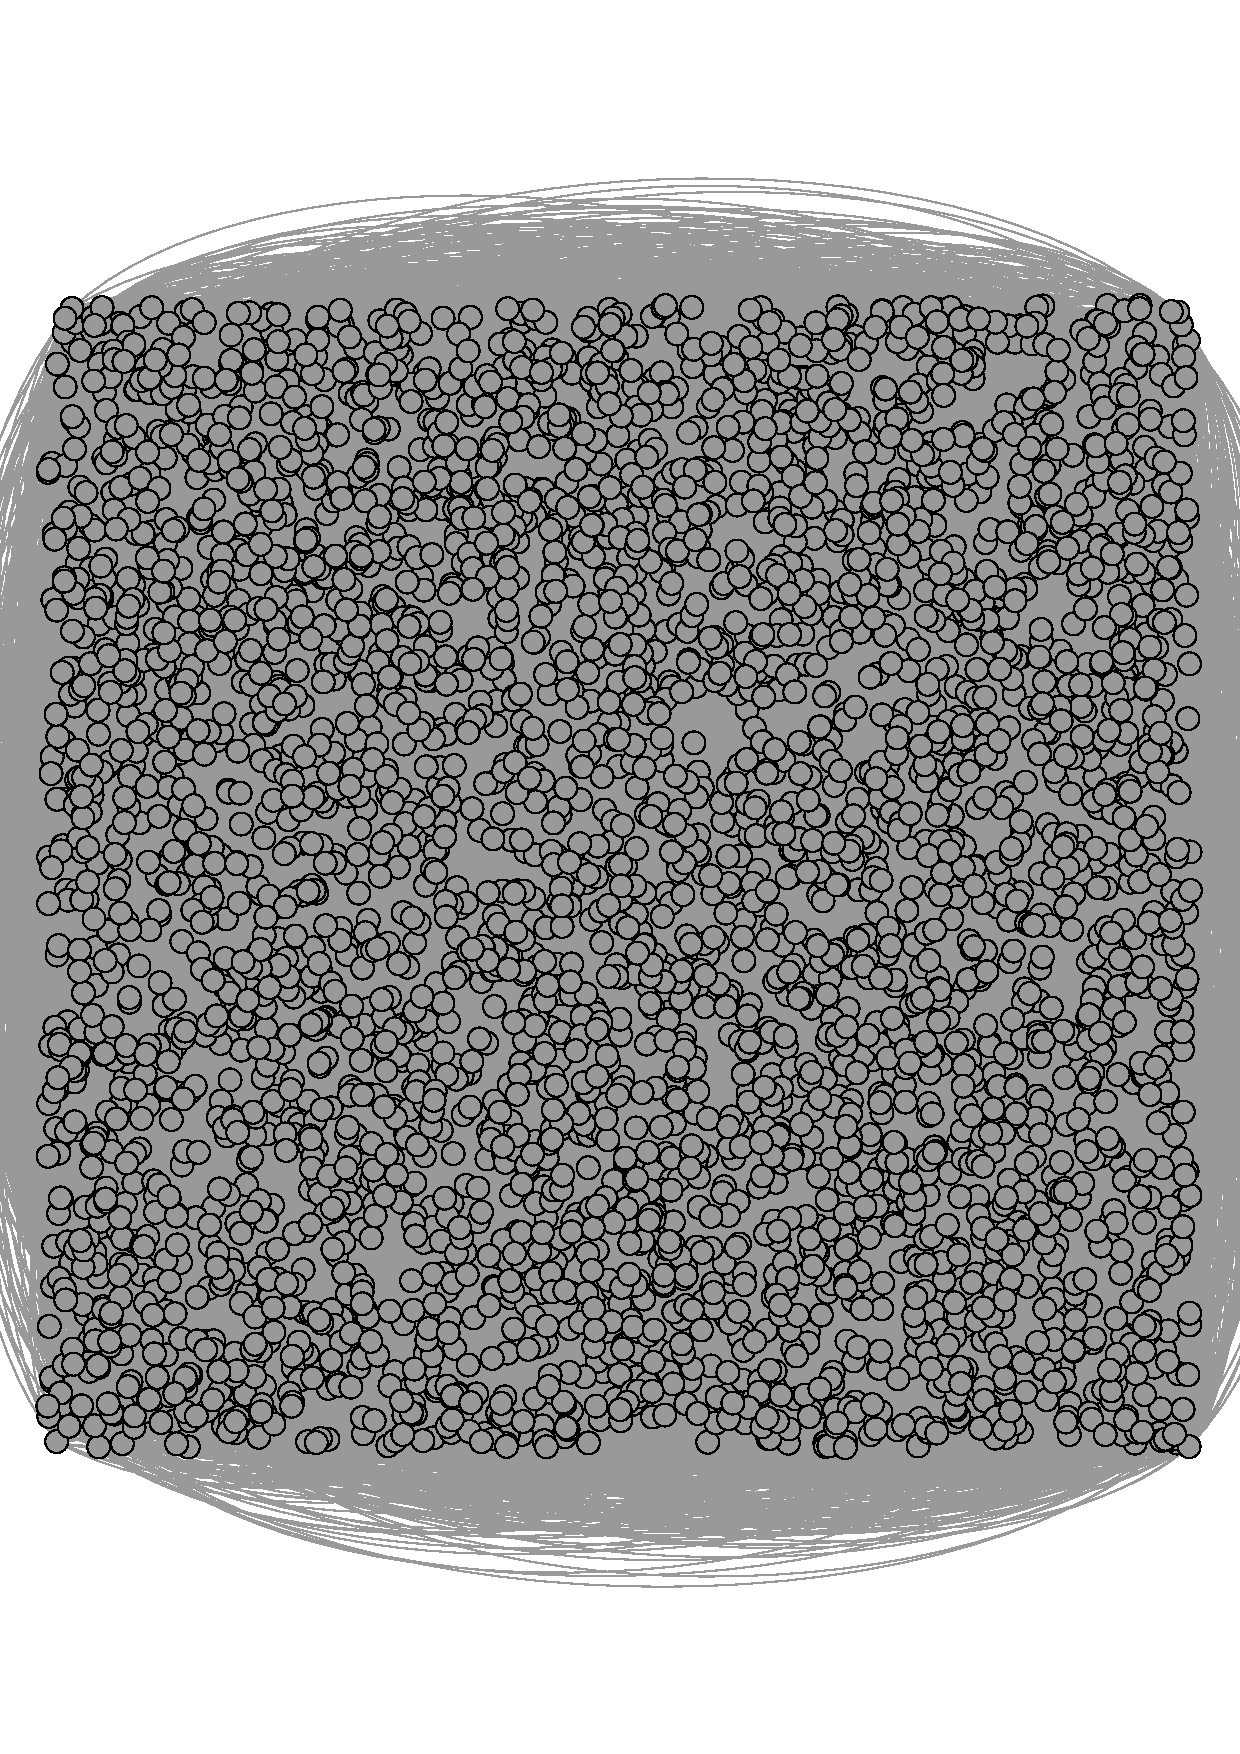
\includegraphics[height=8cm]{includes/gephi1}
%    \caption{Grafik direkt nach Import der Daten}
%    \label{fig:gephi1}
%\end{figure}
%
%\begin{figure}[ht]
%    \centering
%    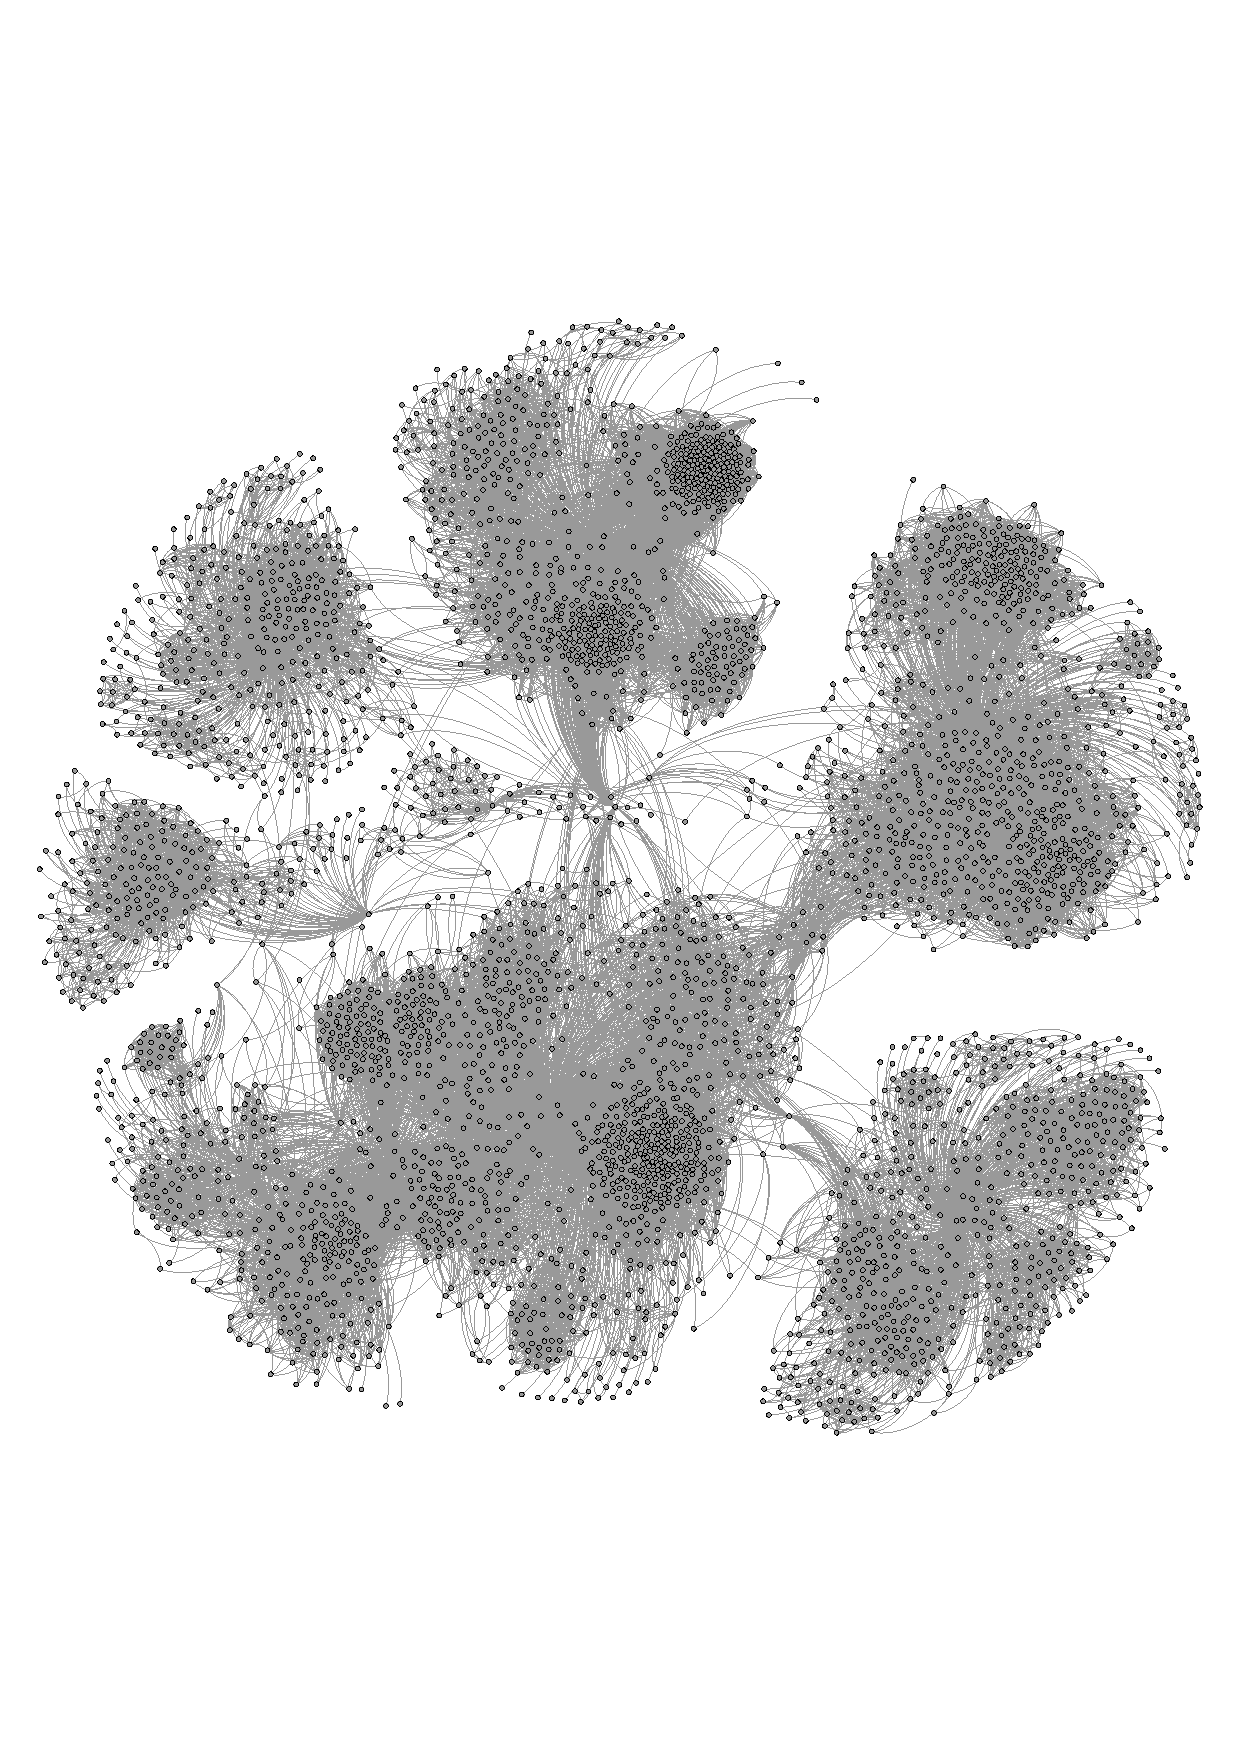
\includegraphics[height=8cm]{includes/gephi2}
%    \caption{Grafik direkt nach Import der Daten}
%    \label{fig:gephi2}
%\end{figure}

Für die Visualisierungen mit Gephi wird hier der Datensatz der Facebook-Freundschaften der empfohlenen Seite verwendet, der aus 10 Netzwerken zusammengesetzt wurde \footnote{Größere Datensätze waren im CIP-Pool leider nicht zu importieren. Selbst mit diesem relativ kleinen Datensatz gab es immer wieder Probleme mit dem begrenzten Speicherplatz. Auf meinem Windows-PC wollte Gephi leider nicht starten.}.

Gephi beginnt nach dem Import des Datensatzes mit einem zufälligen Layout, das die Knoten innerhalb einer rechteckigen Fläche anordnet, siehe \cref{fig:start}. In dieser Darstellung sind bei Datensätzen solcher Größe vermutlich selten Aussagen über die Daten zu treffen.

\begin{figure}[ht]
    \centering
    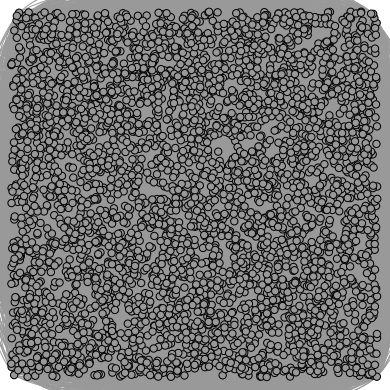
\includegraphics[height=8cm]{includes/snapshot_start}
    \caption{Grafik direkt nach Import der Daten}
    \label{fig:start}
\end{figure}

In erster Linie kann die Visualisierung durch ein Layout verbessert werden, das nach den Beziehungen zwischen den Daten ausgerichtet ist. Die Erfahrung zeigt, dass oft eine Kombination verschiedener Algorithmen ästhetischere Abbildungen ergibt, aus denen bereits erste Erkenntnisse gewonnen werden können. \Cref{fig:einfarbig} zeigt ein solches Layout.

\begin{figure}[ht]
    \centering
    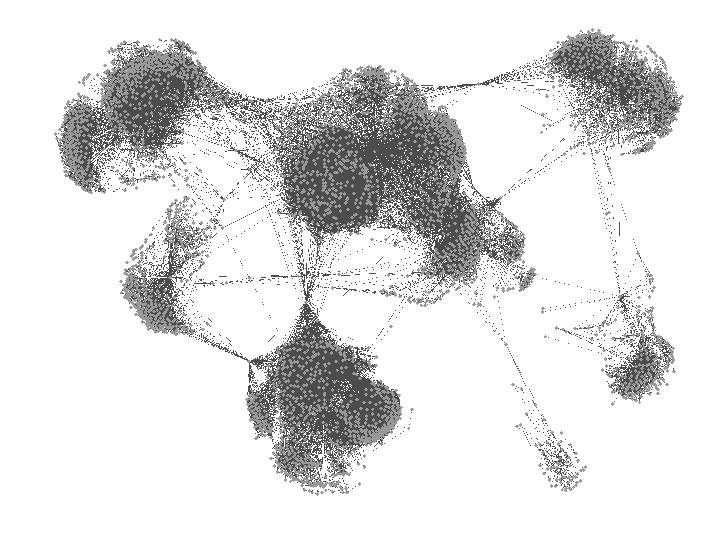
\includegraphics[height=8cm]{includes/snapshot_einfarbig}
    \caption{Grafik nach Anwendung von Layout-Algorithmen}
    \label{fig:einfarbig}
\end{figure}

Zusätzlich können Knoten und Kanten noch eingefärbt werden. Zu den zahlreichen Möglichkeiten gehören unter anderem (Ein-/Ausgangs-)Grad, Kantengewicht oder Zentralitätsmaße. Am nützlichsten hat sich für diesen Datensatz die Färbung der Knoten nach \emph{Modularity} erwiesen, wie in \cref{fig:bunt} zu sehen.

\begin{figure}[ht]
    \centering
    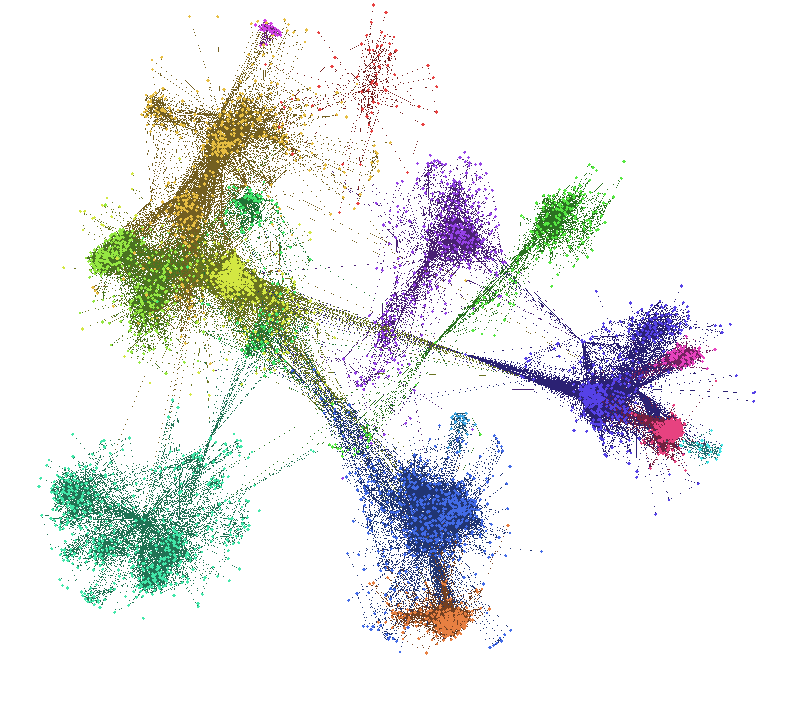
\includegraphics[height=8cm]{includes/snapshot_bunt}
    \caption{Grafik nach Anwendung von Layout-Algorithmen und Einfärben der Knoten}
    \label{fig:bunt}
\end{figure}
\end{document}
